\documentclass[tikz,convert={density=300,outext=.png}]{standalone}
\usepackage{amsmath}
\usetikzlibrary{arrows.meta,graphs}
\begin{document}
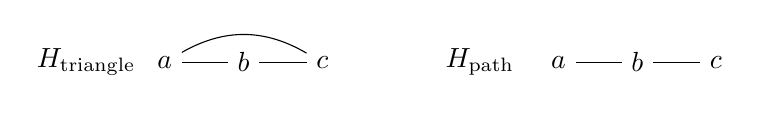
\begin{tikzpicture}
  \node (l) at (-1,0) {$H_{\text{triangle}}$};
    \node (a) at (0,0) {$a$};
    \node (b) at (1,0) {$b$};
    \node (c) at (2,0) {$c$};
  \graph[use existing nodes] {
    a -- b -- c;
    a --[bend left] c;
  };
  \node (l) at (4,0) {$H_{\text{path}}$};
    \node (a) at (5,0) {$a$};
    \node (b) at (6,0) {$b$};
    \node (c) at (7,0) {$c$};
  \graph[use existing nodes] {
    a -- b -- c;
  };
\end{tikzpicture}
\end{document}

